\section{Conclusion and Learnings} \label{section:luckypatcher-learnings}


Results for applications, was ist wenn auf handy ohne store/mit store root/ohne root etc - ringschluss blackmarket da man installieren kann


\begin{table}[h]
\centering
\begin{tabular}{llll}
                                             & \multicolumn{3}{c}{Application}             \\
\multicolumn{1}{c|}{Modus}                   & LicenseTester & Runtastic Pro & Teamspeak 3 \\ \hline
\multicolumn{1}{l|}{Purchased}               & yes           & yes           & yes         \\
\multicolumn{1}{l|}{Pirated}                 & no            & no            & no          \\
\multicolumn{1}{l|}{Auto}                    & yes           & yes           & no          \\
\multicolumn{1}{l|}{Auto (Inversed)}         & no            & yes           & no          \\
\multicolumn{1}{l|}{Extreme}                 & no            & yes           & no          \\
\multicolumn{1}{l|}{Auto+Extreme}            & yes           & yes           & no          \\
\multicolumn{1}{l|}{Auto (Inversed)+Extreme} & no            & yes           & no
\end{tabular}
\caption{Functionality for the test apps before and after patching}
\label{table:functionality}
\end{table}

lvl cracked app was always workign (test)

Amazon cracked app was always working (no client needed)
samsung app also working

applies it directly to the librabry since first patching point could be the initial call, in case modified lvl patching initial call would be not enough since the on success block could contain important code (like ui creation) then it would be useless, target on specific points where decisions are made to alter as few code as possible

since automated customizations have to be implemented to trick it
make false checks to detect tampering -see- user patch

amazon/samsung not much to do since from company, beyond control of developer since injection after developer and a library provided by samsung which is only called, that is why the following not simple methods target lvl

known bytecode patterns, replace with custom, makes mechanism useless

following present ways of protecting against patching attempts, especially predefined recipes circumventing the LVL
high motivation, the patterns/patching modes cover many apps, more than custom

should not use one but many methods
solution for current version of lucky patcher, future might be different, arms race scenario
\cite{munteanLicense}
%

\begin{figure}[h]
    \centering
    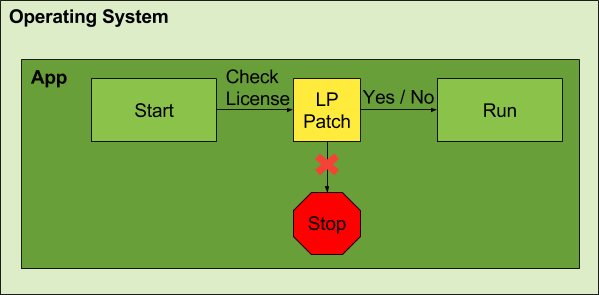
\includegraphics[width=0.8\textwidth]{data/verificationNowAttack.png}
    \caption{Abstraction of the current attack on the license verification mechanism}
    \label{fig:verificationNowAttack}
\end{figure}


Aamzon + Samsung
Wenn man sich slide.me anschaut, ist dies eine simple Variante von Zirconia und ist theoretisch noch einfacher zu cracken. Anstatt auf einen Callback zu setzen welchen man in der jar modifizieren müsste, kann man bei slide.me einfach den Code Block
 if(someRights != null){
        // you have granted rights.
    } else {
        // You don't have any rights for the feature in cause. Try
        // some features. (Currently not supporting multiple 'features')
    }
modifizieren und immer in den "you have granted rights" Block springen. Dies ist besonders einfach, da durch die statische jar auch kein modifiziertes Verhalten zu erwarten ist.


nur ja/nein test bzw ergebnis zuweisung und drauf folgender test kann IMMER geskippt werden, vergleich figure~\ref{fig:verificationNow}



fügt keinen code hinzu sondern ersetzt commands => checksum/signature
